\documentclass[a4paper]{article}

\usepackage{fullpage}
\usepackage{parskip}
\usepackage{tikz}
\usepackage{amsmath}
\usepackage{amsfonts}
\usepackage{amssymb}
\usepackage{hyperref}
\usepackage[utf8]{inputenc}

\newtheorem{theorem}{Theorem}
\newtheorem{lemma}{Lemma}

\title{Title}
\author{André Graubner, Lukas Walker, Leonard von Kleist}
\date{1969/07/20}

\begin{document} 

\maketitle

\section{Aufgabe 7b}

	Hier speichert jeder Zustand die Differenz 
	$(\lvert w \rvert_a + 2\lvert w \rvert_b)\mod{4}  - (3 \cdot \lvert w \rvert)\mod{4}$:

\begin{center}
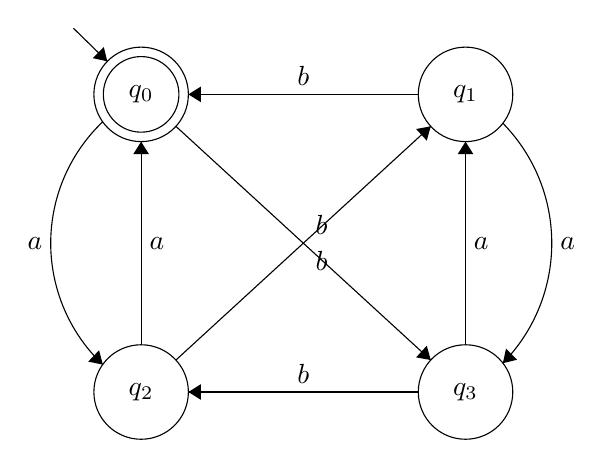
\begin{tikzpicture}[scale=0.2]
\tikzstyle{every node}+=[inner sep=0pt]
\draw [black] (19.7,-17.9) circle (3);
\draw (19.7,-17.9) node {$q_0$};
\draw [black] (19.7,-17.9) circle (2.4);
\draw [black] (40.3,-17.9) circle (3);
\draw (40.3,-17.9) node {$q_1$};
\draw [black] (19.7,-36.8) circle (3);
\draw (19.7,-36.8) node {$q_2$};
\draw [black] (40.3,-36.8) circle (3);
\draw (40.3,-36.8) node {$q_3$};
\draw [black] (17.266,-35.063) arc (-133.57878:-226.42122:10.648);
\fill [black] (17.27,-35.06) -- (17.03,-34.15) -- (16.34,-34.87);
\draw (13.46,-27.35) node [left] {$a$};
\draw [black] (19.7,-33.8) -- (19.7,-20.9);
\fill [black] (19.7,-20.9) -- (19.2,-21.7) -- (20.2,-21.7);
\draw (20.2,-27.35) node [right] {$a$};
\draw [black] (42.666,-19.729) arc (44.40083:-44.40083:10.892);
\fill [black] (42.67,-34.97) -- (43.58,-34.75) -- (42.87,-34.05);
\draw (46.28,-27.35) node [right] {$a$};
\draw [black] (40.3,-33.8) -- (40.3,-20.9);
\fill [black] (40.3,-20.9) -- (39.8,-21.7) -- (40.8,-21.7);
\draw (40.8,-27.35) node [right] {$a$};
\draw [black] (37.3,-17.9) -- (22.7,-17.9);
\fill [black] (22.7,-17.9) -- (23.5,-18.4) -- (23.5,-17.4);
\draw (30,-17.4) node [above] {$b$};
\draw [black] (37.3,-36.8) -- (22.7,-36.8);
\fill [black] (22.7,-36.8) -- (23.5,-37.3) -- (23.5,-36.3);
\draw (30,-36.3) node [above] {$b$};
\draw [black] (21.91,-34.77) -- (38.09,-19.93);
\fill [black] (38.09,-19.93) -- (37.16,-20.1) -- (37.84,-20.84);
\draw (31.16,-27.84) node [below] {$b$};
\draw [black] (21.91,-19.93) -- (38.09,-34.77);
\fill [black] (38.09,-34.77) -- (37.84,-33.86) -- (37.16,-34.6);
\draw (31.16,-26.86) node [above] {$b$};
\draw [black] (15.4,-13.7) -- (17.55,-15.8);
\fill [black] (17.55,-15.8) -- (17.33,-14.89) -- (16.63,-15.6);
\end{tikzpicture}
\end{center}

\begin{enumerate}
\item
$Kl\big[q_0\big] = \Big\{w \in \big\{a,b\big\}^* \mid 
(\lvert w \rvert_a + 2\lvert w \rvert_b)\mod{4} - (3 \cdot \lvert w \rvert)\mod{4} = 0\Big\}$
\item
$Kl\big[q_1\big] = \Big\{w \in \big\{a,b\big\}^* \mid 
(\lvert w \rvert_a + 2\lvert w \rvert_b)\mod{4} - (3 \cdot \lvert w \rvert)\mod{4} = 1    \Big\}$
\item
$Kl\big[q_2\big] = \Big\{w \in \big\{a,b\big\}^* \mid 
(\lvert w \rvert_a + 2\lvert w \rvert_b)\mod{4} - (3 \cdot \lvert w \rvert)\mod{4} = 2    \Big\}$
\item
$Kl\big[q_3\big] = \Big\{w \in \big\{a,b\big\}^* \mid 
(\lvert w \rvert_a + 2\lvert w \rvert_b)\mod{4} - (3 \cdot \lvert w \rvert)\mod{4} = 3    \Big\}$
\end{enumerate}
\end{document}
